% Options for packages loaded elsewhere
\PassOptionsToPackage{unicode}{hyperref}
\PassOptionsToPackage{hyphens}{url}
%
\documentclass[
]{book}
\title{My First Steps in Neuronal Networks\\
(Beginners Guide)}
\author{Axel Roth}
\date{2021-11-07}

\usepackage{amsmath,amssymb}
\usepackage{lmodern}
\usepackage{iftex}
\ifPDFTeX
  \usepackage[T1]{fontenc}
  \usepackage[utf8]{inputenc}
  \usepackage{textcomp} % provide euro and other symbols
\else % if luatex or xetex
  \usepackage{unicode-math}
  \defaultfontfeatures{Scale=MatchLowercase}
  \defaultfontfeatures[\rmfamily]{Ligatures=TeX,Scale=1}
\fi
% Use upquote if available, for straight quotes in verbatim environments
\IfFileExists{upquote.sty}{\usepackage{upquote}}{}
\IfFileExists{microtype.sty}{% use microtype if available
  \usepackage[]{microtype}
  \UseMicrotypeSet[protrusion]{basicmath} % disable protrusion for tt fonts
}{}
\makeatletter
\@ifundefined{KOMAClassName}{% if non-KOMA class
  \IfFileExists{parskip.sty}{%
    \usepackage{parskip}
  }{% else
    \setlength{\parindent}{0pt}
    \setlength{\parskip}{6pt plus 2pt minus 1pt}}
}{% if KOMA class
  \KOMAoptions{parskip=half}}
\makeatother
\usepackage{xcolor}
\IfFileExists{xurl.sty}{\usepackage{xurl}}{} % add URL line breaks if available
\IfFileExists{bookmark.sty}{\usepackage{bookmark}}{\usepackage{hyperref}}
\hypersetup{
  pdfauthor={Axel Roth},
  hidelinks,
  pdfcreator={LaTeX via pandoc}}
\urlstyle{same} % disable monospaced font for URLs
\usepackage{color}
\usepackage{fancyvrb}
\newcommand{\VerbBar}{|}
\newcommand{\VERB}{\Verb[commandchars=\\\{\}]}
\DefineVerbatimEnvironment{Highlighting}{Verbatim}{commandchars=\\\{\}}
% Add ',fontsize=\small' for more characters per line
\usepackage{framed}
\definecolor{shadecolor}{RGB}{248,248,248}
\newenvironment{Shaded}{\begin{snugshade}}{\end{snugshade}}
\newcommand{\AlertTok}[1]{\textcolor[rgb]{0.94,0.16,0.16}{#1}}
\newcommand{\AnnotationTok}[1]{\textcolor[rgb]{0.56,0.35,0.01}{\textbf{\textit{#1}}}}
\newcommand{\AttributeTok}[1]{\textcolor[rgb]{0.77,0.63,0.00}{#1}}
\newcommand{\BaseNTok}[1]{\textcolor[rgb]{0.00,0.00,0.81}{#1}}
\newcommand{\BuiltInTok}[1]{#1}
\newcommand{\CharTok}[1]{\textcolor[rgb]{0.31,0.60,0.02}{#1}}
\newcommand{\CommentTok}[1]{\textcolor[rgb]{0.56,0.35,0.01}{\textit{#1}}}
\newcommand{\CommentVarTok}[1]{\textcolor[rgb]{0.56,0.35,0.01}{\textbf{\textit{#1}}}}
\newcommand{\ConstantTok}[1]{\textcolor[rgb]{0.00,0.00,0.00}{#1}}
\newcommand{\ControlFlowTok}[1]{\textcolor[rgb]{0.13,0.29,0.53}{\textbf{#1}}}
\newcommand{\DataTypeTok}[1]{\textcolor[rgb]{0.13,0.29,0.53}{#1}}
\newcommand{\DecValTok}[1]{\textcolor[rgb]{0.00,0.00,0.81}{#1}}
\newcommand{\DocumentationTok}[1]{\textcolor[rgb]{0.56,0.35,0.01}{\textbf{\textit{#1}}}}
\newcommand{\ErrorTok}[1]{\textcolor[rgb]{0.64,0.00,0.00}{\textbf{#1}}}
\newcommand{\ExtensionTok}[1]{#1}
\newcommand{\FloatTok}[1]{\textcolor[rgb]{0.00,0.00,0.81}{#1}}
\newcommand{\FunctionTok}[1]{\textcolor[rgb]{0.00,0.00,0.00}{#1}}
\newcommand{\ImportTok}[1]{#1}
\newcommand{\InformationTok}[1]{\textcolor[rgb]{0.56,0.35,0.01}{\textbf{\textit{#1}}}}
\newcommand{\KeywordTok}[1]{\textcolor[rgb]{0.13,0.29,0.53}{\textbf{#1}}}
\newcommand{\NormalTok}[1]{#1}
\newcommand{\OperatorTok}[1]{\textcolor[rgb]{0.81,0.36,0.00}{\textbf{#1}}}
\newcommand{\OtherTok}[1]{\textcolor[rgb]{0.56,0.35,0.01}{#1}}
\newcommand{\PreprocessorTok}[1]{\textcolor[rgb]{0.56,0.35,0.01}{\textit{#1}}}
\newcommand{\RegionMarkerTok}[1]{#1}
\newcommand{\SpecialCharTok}[1]{\textcolor[rgb]{0.00,0.00,0.00}{#1}}
\newcommand{\SpecialStringTok}[1]{\textcolor[rgb]{0.31,0.60,0.02}{#1}}
\newcommand{\StringTok}[1]{\textcolor[rgb]{0.31,0.60,0.02}{#1}}
\newcommand{\VariableTok}[1]{\textcolor[rgb]{0.00,0.00,0.00}{#1}}
\newcommand{\VerbatimStringTok}[1]{\textcolor[rgb]{0.31,0.60,0.02}{#1}}
\newcommand{\WarningTok}[1]{\textcolor[rgb]{0.56,0.35,0.01}{\textbf{\textit{#1}}}}
\usepackage{longtable,booktabs,array}
\usepackage{calc} % for calculating minipage widths
% Correct order of tables after \paragraph or \subparagraph
\usepackage{etoolbox}
\makeatletter
\patchcmd\longtable{\par}{\if@noskipsec\mbox{}\fi\par}{}{}
\makeatother
% Allow footnotes in longtable head/foot
\IfFileExists{footnotehyper.sty}{\usepackage{footnotehyper}}{\usepackage{footnote}}
\makesavenoteenv{longtable}
\usepackage{graphicx}
\makeatletter
\def\maxwidth{\ifdim\Gin@nat@width>\linewidth\linewidth\else\Gin@nat@width\fi}
\def\maxheight{\ifdim\Gin@nat@height>\textheight\textheight\else\Gin@nat@height\fi}
\makeatother
% Scale images if necessary, so that they will not overflow the page
% margins by default, and it is still possible to overwrite the defaults
% using explicit options in \includegraphics[width, height, ...]{}
\setkeys{Gin}{width=\maxwidth,height=\maxheight,keepaspectratio}
% Set default figure placement to htbp
\makeatletter
\def\fps@figure{htbp}
\makeatother
\setlength{\emergencystretch}{3em} % prevent overfull lines
\providecommand{\tightlist}{%
  \setlength{\itemsep}{0pt}\setlength{\parskip}{0pt}}
\setcounter{secnumdepth}{5}
\usepackage{booktabs}
\usepackage{amsthm}
\makeatletter
\def\thm@space@setup{%
  \thm@preskip=8pt plus 2pt minus 4pt
  \thm@postskip=\thm@preskip
}
\makeatother
\ifLuaTeX
  \usepackage{selnolig}  % disable illegal ligatures
\fi
\usepackage[]{natbib}
\bibliographystyle{apalike}

\begin{document}
\maketitle

{
\setcounter{tocdepth}{1}
\tableofcontents
}
\hypertarget{about}{%
\chapter{About}\label{about}}

\hypertarget{me}{%
\section{Me}\label{me}}

Hello, my name is Axel Roth and im studding math at a master degree in germany. In the same moment im working half-time in the finance field and programming in a wide range of tasks like index replication, factormodels, data visualisation, datamanagement, shiny applications, documantations with rmarkdown, building internal packages and much more. So the most of my experience i gained was around R and all its features. And now the interesting question\ldots{} Why do i want to write a beginners guide in the field of Neuronal Networks?\\
Its simple, at the moment i have a lecture in that we learn how to program a Neuronal Network from scratch with basic packages from python and i want to share my experience. Additionaly i learned all i know from free sources of the internet and thats why i want to give something back. Furthermore its a good use-case to write my first things in english and test the fancy Bookdown and GitBook features.

\hypertarget{the-book}{%
\section{The Book}\label{the-book}}

This Book will be more or the less the documentation of my lecture ``Finance Project'' in that we learn to program a simple Perceptron (the simplest Neuronal Network) and then we will continue with a multi layer Perceptron and finish with a slight insight into decision trees. On this journey, we will test the Neuronal Network in different examples that are easy to reproduce. Because these are my first steps in this field, i need to appolagice for my terrible spelling and cant guarantee you the best quality, but maybe this is the best way to educate and attract unexperienced readers to have a look into this field.

\hypertarget{how-it-works}{%
\section{How it works}\label{how-it-works}}

Im coding this book in the IDE R-Studio with the framework of Bookdown and embed python code that is made possible by the reticulate package. Thats why i need to load the python interpreter in the following R-chunk:

\begin{Shaded}
\begin{Highlighting}[]
\FunctionTok{library}\NormalTok{(reticulate)}
\FunctionTok{Sys.setenv}\NormalTok{(}\AttributeTok{RETICULATE\_PYTHON =} \StringTok{"D:}\SpecialCharTok{\textbackslash{}\textbackslash{}}\StringTok{WinPython2}\SpecialCharTok{\textbackslash{}\textbackslash{}}\StringTok{WPy64{-}3950}\SpecialCharTok{\textbackslash{}\textbackslash{}}\StringTok{python{-}3.9.5.amd64}\SpecialCharTok{\textbackslash{}\textbackslash{}}\StringTok{"}\NormalTok{)}
\end{Highlighting}
\end{Shaded}

Additionaly im using a fully portable version of R-Studio, R and python. Its nice to have if you want to switch for example between university PCs and your own. R-Studio supports it and python can be downloaded via WinPython to be fully portable.

\hypertarget{single-perceptron}{%
\chapter{Single Perceptron}\label{single-perceptron}}

In this chapter i will teach you how to code a single Perceptron in python with only the numpy package. Numpy uses a vectorizible math structure in which you can easily calculate elementwise or do stuff like normal matrix multiplications with just a symbol (i always interpret Vectors as one dimensional matrices!). At the most of the time, its just translating math formulas into python code without changing its structure.\\
First of all we are starting with the needed parameters, that are explained later:

Number of runs over the training data := \texttt{n\_train}\\
Learning rate := \(\alpha =\) \texttt{alpha}\\
Bias value := \(\beta =\) \texttt{bias}
and the activation function:\\
\[ 
step(s)= 
\begin{cases}
    1,& s   \geq \beta\\
    0,& s < \beta
\end{cases}
\]
This function is named the heavyside-function and should be the easiest activation function to start with. If the weighted sum is smaller than the \texttt{bias} it will send the value zero to the next neuron. Our brain works with the same behavior. If the electricity is too small, the neuron will not activate and the next one dosent get any electricity.

The traings dataset is the following:
\[
\left[
\begin{array}{cc|c}
x_i,_1 & x_i,_2 & y_i \\
\end{array}
\right]
\]
\[
\left[
\begin{array}{cc|c}
0 & 0 & 0 \\
0 & 1 & 1 \\
1 & 0 & 1 \\
1 & 1 & 1 \\
\end{array}
\right]
\]
The provided training dataset contains the \texttt{X} matrix with two inputs for each scenario and the \texttt{Y} matrix with the correct output. If your looking exactly you can see that this is the OR-Gate. Later you will see why these type of problems are the only suitable things to do with a single neuron.

The needed python imports and default options are the following:

\begin{Shaded}
\begin{Highlighting}[]
\ImportTok{import}\NormalTok{ numpy }\ImportTok{as}\NormalTok{ np}
\ImportTok{import}\NormalTok{ random }\ImportTok{as}\NormalTok{ ra}
\ImportTok{import}\NormalTok{ pandas }\ImportTok{as}\NormalTok{ pd}
\ImportTok{import}\NormalTok{ matplotlib.pyplot }\ImportTok{as}\NormalTok{ pyplot}
\NormalTok{pd.set\_option(}\StringTok{\textquotesingle{}display.max\_rows\textquotesingle{}}\NormalTok{, }\DecValTok{500}\NormalTok{)}
\NormalTok{pd.set\_option(}\StringTok{\textquotesingle{}display.max\_columns\textquotesingle{}}\NormalTok{, }\DecValTok{500}\NormalTok{)}
\NormalTok{pd.set\_option(}\StringTok{\textquotesingle{}display.width\textquotesingle{}}\NormalTok{, }\DecValTok{1000}\NormalTok{)}
\end{Highlighting}
\end{Shaded}

( Do you see more imports than only the numpy package? \href{https://www.youtube.com/watch?v=dQw4w9WgXcQ}{Yes} or No )

Now that we have all the needed parameters and settings, i can give you a quick overview of the algorithm.

\hypertarget{neural-network-basics}{%
\section{Neural Network Basics}\label{neural-network-basics}}

In a NN we are having two basic parts, the forward pass and the backward pass. In the forward pass we are calculating the weighted sum of each input with its weights of the layer and evaluating the activation function with it, to calculate the output. In the backward pass we are analyzing the error to adjust the weights accordingly. This is it! This is all a NN will do. I explained everything to you. Have a good life\ldots{}\\
Ahh no no ok we have a look deeper into it :)

Whats exactly is the forward pass in a single Perceptron? Its just the evaluation of the acvtivation function with the weighted sum like i said, so you have (with the matrix dimensions included) for one scenario out of the training dataset, the following:
\[
  step(W^{(1,2)} \cdot x^{(2,1)}) = y^{(1,1)}
\]
That is the normal approach to iterate over all scenarios in the training dataset\ldots{}\\
But i think its not the right way to describe it, because it gets very confusing to interpret it for all scenarios.

My next approach is to consider all scenarios in the training dataset in one formula. If your data isnt that huge, its a much faster approach as well. First of all we need to interpret the new dimensions of \(W\) and \(X\).\\
We have \(X\) as:
\[
  X = \left[
  \begin{array}{cc}
  0 & 0 \\
  0 & 1 \\
  1 & 0 \\
  1 & 1 \\
  \end{array}
  \right]
\]
each row describes the inputs for each neuron in the scenario \(i\).\\
For the weights \(W\) we have for example:
\[
  W =\left[
  \begin{array}{c}
  0.1 \\ 
  0.2 \\ 
  \end{array}
  \right]
\]
The new formular looks like this:
\[
  step(X \cdot W) = Y
\]
For example if you take a look at the \(i\)-th row or scenario of \(X\) you will see the following:
\[
  Y_i,_0 = step([X_i,_0 \cdot W_0,_0 + X_i,_1 \cdot W_1,_0 ])
\]
and \(Y_i,_0\) is the approximated output of the \(i\)-th scenario. Now we can look at the NN and compare the formula with it:\\
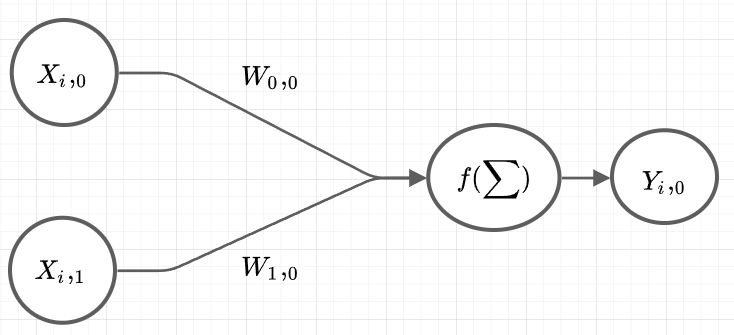
\includegraphics[width=0.5\textwidth,height=\textheight]{./img/NN_01_v4.png}

Yes it is the same, its the weighted sum of the inputs and evaluated the activation function with it to calculate the output of the scenario \(i\).

\hypertarget{forward-pass}{%
\section{Forward pass}\label{forward-pass}}

Now we create the so called \texttt{forward()} function in python:

\begin{Shaded}
\begin{Highlighting}[]
\KeywordTok{def}\NormalTok{ forward(X, W):}
  \ControlFlowTok{return}\NormalTok{( step(X }\OperatorTok{@}\NormalTok{ W) )}
\end{Highlighting}
\end{Shaded}

(Numpy provides us with the \texttt{@} symbol to make a matrix multiplication and the \texttt{.T} to transpose)

Because we want to put one dimensional matrices into the \texttt{step()} function we need to use numpy for the if-else statement:

\begin{Shaded}
\begin{Highlighting}[]
\KeywordTok{def}\NormalTok{ step(s):}
  \ControlFlowTok{return}\NormalTok{( np.where(s }\OperatorTok{\textgreater{}=}\NormalTok{ bias, }\DecValTok{1}\NormalTok{, }\DecValTok{0}\NormalTok{) )}
\end{Highlighting}
\end{Shaded}

Here an small example for the forward pass:

\begin{Shaded}
\begin{Highlighting}[]
\NormalTok{X }\OperatorTok{=}\NormalTok{ np.array([}
\NormalTok{  [}\DecValTok{0}\NormalTok{,}\DecValTok{0}\NormalTok{],}
\NormalTok{  [}\DecValTok{0}\NormalTok{,}\DecValTok{1}\NormalTok{],}
\NormalTok{  [}\DecValTok{1}\NormalTok{,}\DecValTok{0}\NormalTok{],}
\NormalTok{  [}\DecValTok{1}\NormalTok{,}\DecValTok{1}\NormalTok{],}
\NormalTok{])}
\NormalTok{W }\OperatorTok{=}\NormalTok{ np.array([}
\NormalTok{  [}\FloatTok{0.1}\NormalTok{], }
\NormalTok{  [}\FloatTok{0.2}\NormalTok{]}
\NormalTok{])}
\NormalTok{bias }\OperatorTok{=} \DecValTok{1}
\NormalTok{Y\_approx }\OperatorTok{=}\NormalTok{ forward(X, W)}
\BuiltInTok{print}\NormalTok{(Y\_approx)}
\end{Highlighting}
\end{Shaded}

\begin{verbatim}
## [[0]
##  [0]
##  [0]
##  [0]]
\end{verbatim}

And these are all the generated outputs of our NN over all scenarios. Now we need to calculate the error and adjust the weights accordingly.

\hypertarget{backward-pass}{%
\section{backward pass}\label{backward-pass}}

To adjust the weights in a single Perceptron, we need the Delta-Rule:
\[
  W(t+1) = W(t) + \Delta W(t)
\]
with
\[
  \Delta W(t) = \alpha \cdot X^{T} \cdot (Y - \hat{Y})
\]
and \(\hat{Y}\) is the output of the NN.

\begin{Shaded}
\begin{Highlighting}[]
\KeywordTok{def}\NormalTok{ backward(W, X, Y, alpha, Y\_approx):}
    \ControlFlowTok{return}\NormalTok{(W }\OperatorTok{+}\NormalTok{ alpha }\OperatorTok{*}\NormalTok{ X.T }\OperatorTok{@}\NormalTok{ (Y }\OperatorTok{{-}}\NormalTok{ Y\_approx))}
\end{Highlighting}
\end{Shaded}

with the result of the forward pass and example data we have the following:

\begin{Shaded}
\begin{Highlighting}[]
\NormalTok{Y }\OperatorTok{=}\NormalTok{ np.array([}
\NormalTok{  [}\DecValTok{0}\NormalTok{],}
\NormalTok{  [}\DecValTok{1}\NormalTok{],}
\NormalTok{  [}\DecValTok{1}\NormalTok{],}
\NormalTok{  [}\DecValTok{1}\NormalTok{]}
\NormalTok{])}
\NormalTok{alpha }\OperatorTok{=} \FloatTok{0.01}
\NormalTok{W }\OperatorTok{=}\NormalTok{ backward(W, X, Y, alpha, Y\_approx)}
\BuiltInTok{print}\NormalTok{(W)}
\end{Highlighting}
\end{Shaded}

\begin{verbatim}
## [[0.12]
##  [0.22]]
\end{verbatim}

and this is the new weight.

\hypertarget{single-perceptron-1}{%
\section{Single Perceptron}\label{single-perceptron-1}}

Now we want to do the same process multiple times, to train the NN:

\begin{Shaded}
\begin{Highlighting}[]
\NormalTok{X }\OperatorTok{=}\NormalTok{ np.array([}
\NormalTok{  [}\DecValTok{0}\NormalTok{,}\DecValTok{0}\NormalTok{],}
\NormalTok{  [}\DecValTok{0}\NormalTok{,}\DecValTok{1}\NormalTok{],}
\NormalTok{  [}\DecValTok{1}\NormalTok{,}\DecValTok{0}\NormalTok{],}
\NormalTok{  [}\DecValTok{1}\NormalTok{,}\DecValTok{1}\NormalTok{],}
\NormalTok{])}
\NormalTok{Y }\OperatorTok{=}\NormalTok{ np.array([}
\NormalTok{  [}\DecValTok{0}\NormalTok{],}
\NormalTok{  [}\DecValTok{1}\NormalTok{],}
\NormalTok{  [}\DecValTok{1}\NormalTok{],}
\NormalTok{  [}\DecValTok{1}\NormalTok{]}
\NormalTok{])}
\NormalTok{W }\OperatorTok{=}\NormalTok{ np.array([}
\NormalTok{  [}\FloatTok{0.1}\NormalTok{], }
\NormalTok{  [}\FloatTok{0.2}\NormalTok{]}
\NormalTok{])}
\NormalTok{alpha }\OperatorTok{=} \FloatTok{0.01}
\NormalTok{bias }\OperatorTok{=} \DecValTok{1}
\NormalTok{train\_n }\OperatorTok{=} \DecValTok{100}

\NormalTok{errors }\OperatorTok{=}\NormalTok{ []}
\ControlFlowTok{for}\NormalTok{ i }\KeywordTok{in} \BuiltInTok{range}\NormalTok{(train\_n):}
\NormalTok{  Y\_approx }\OperatorTok{=}\NormalTok{ forward(X, W)}
\NormalTok{  errors.append(Y }\OperatorTok{{-}}\NormalTok{ Y\_approx)}
\NormalTok{  W }\OperatorTok{=}\NormalTok{ backward(W, X, Y, alpha, Y\_approx)}
\end{Highlighting}
\end{Shaded}

The KNN is trained now. Now we want to look at the error. We want to measure the mean-square-error with the following formula:
\[
  Error_i = \frac{1}{2} \cdot \sum(Y-\hat{Y})^2
\]
or as python code:

\begin{Shaded}
\begin{Highlighting}[]
\KeywordTok{def}\NormalTok{ mean\_square\_error(error):}
  \ControlFlowTok{return}\NormalTok{( }\FloatTok{0.5} \OperatorTok{*}\NormalTok{ np.}\BuiltInTok{sum}\NormalTok{(error }\OperatorTok{**} \DecValTok{2}\NormalTok{) )}
\end{Highlighting}
\end{Shaded}

Now we need to calculate the mean-square-error for each element in the list \texttt{errors} which is made with \texttt{map()}:

\begin{Shaded}
\begin{Highlighting}[]
\NormalTok{mean\_square\_errors }\OperatorTok{=}\NormalTok{ np.array(}\BuiltInTok{list}\NormalTok{(}\BuiltInTok{map}\NormalTok{(mean\_square\_error, errors)))}
\end{Highlighting}
\end{Shaded}

To plot the errors, im using the following function:

\begin{Shaded}
\begin{Highlighting}[]
\KeywordTok{def}\NormalTok{ plot\_error(errors, title):}
\NormalTok{  x }\OperatorTok{=} \BuiltInTok{list}\NormalTok{(}\BuiltInTok{range}\NormalTok{(}\BuiltInTok{len}\NormalTok{(errors)))}
\NormalTok{  y }\OperatorTok{=}\NormalTok{ np.array(errors)}
\NormalTok{  pyplot.figure(figsize}\OperatorTok{=}\NormalTok{(}\DecValTok{6}\NormalTok{,}\DecValTok{6}\NormalTok{))}
\NormalTok{  pyplot.plot(x, y, }\StringTok{"g"}\NormalTok{, linewidth}\OperatorTok{=}\DecValTok{1}\NormalTok{)}
\NormalTok{  pyplot.xlabel(}\StringTok{"Iterations"}\NormalTok{, fontsize }\OperatorTok{=} \DecValTok{16}\NormalTok{)}
\NormalTok{  pyplot.ylabel(}\StringTok{"Mean Square Error"}\NormalTok{, fontsize }\OperatorTok{=} \DecValTok{16}\NormalTok{)}
\NormalTok{  pyplot.title(title)}
\NormalTok{  pyplot.ylim(}\OperatorTok{{-}}\FloatTok{0.01}\NormalTok{,}\BuiltInTok{max}\NormalTok{(errors)}\OperatorTok{*}\FloatTok{1.2}\NormalTok{)}
\NormalTok{  pyplot.show()}
  
  
\NormalTok{plot\_error(mean\_square\_errors, }\StringTok{"Mean{-}Square{-}Errors of a single Perceptron"}\NormalTok{)}
\end{Highlighting}
\end{Shaded}

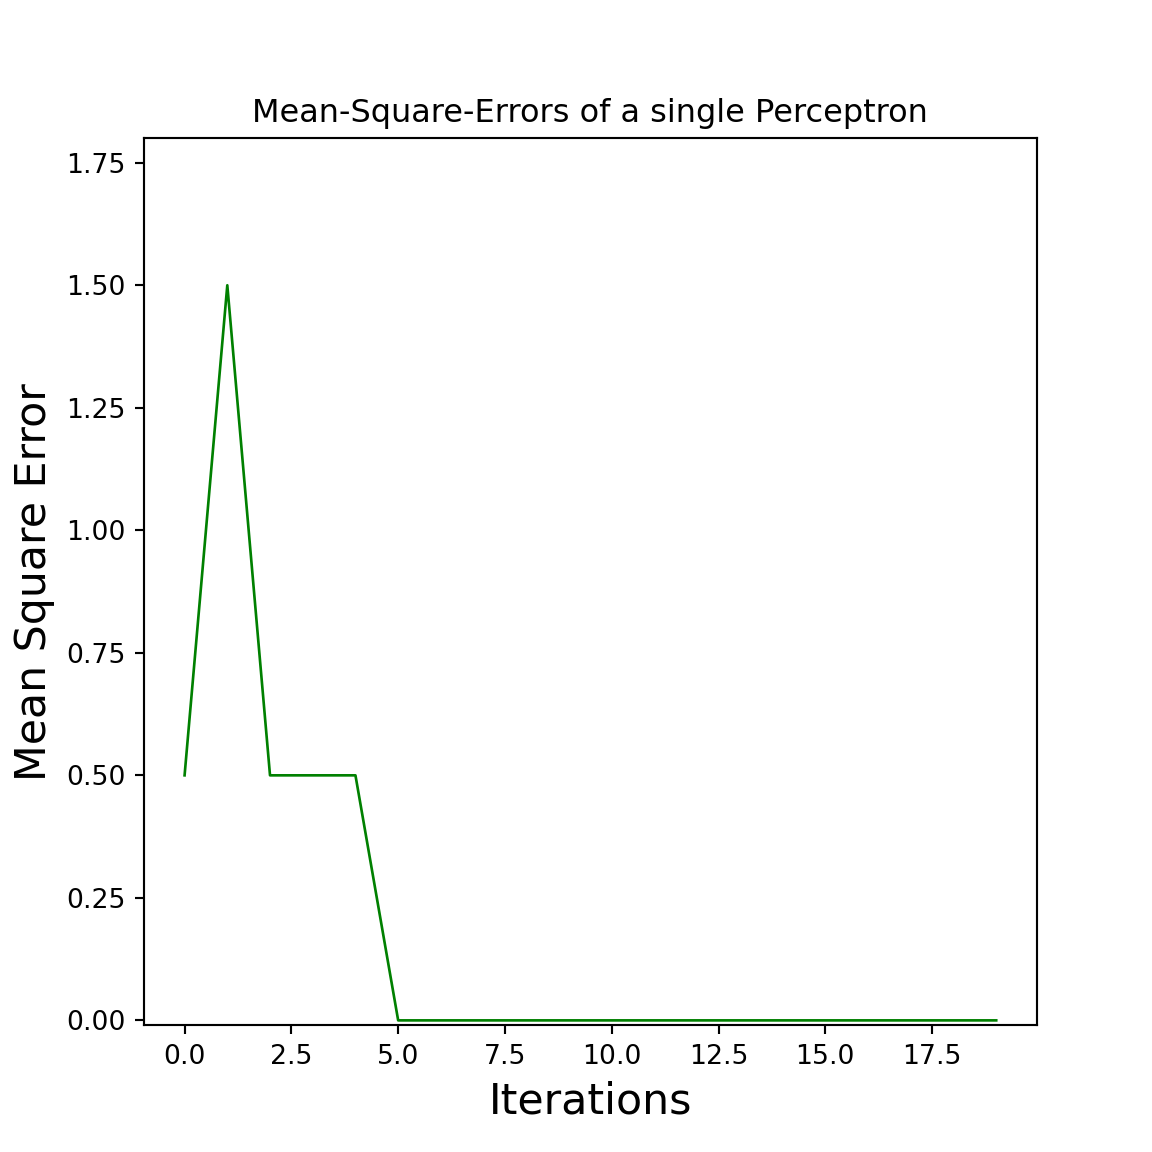
\includegraphics{gitbook-demo_files/figure-latex/unnamed-chunk-11-1.pdf}

If you survived until now, you have learned how you can program a single Perceptron!

\hypertarget{appendix-full-code}{%
\section{Appendix (full code)}\label{appendix-full-code}}

\begin{Shaded}
\begin{Highlighting}[]
\ImportTok{import}\NormalTok{ numpy }\ImportTok{as}\NormalTok{ np}
\ImportTok{import}\NormalTok{ random }\ImportTok{as}\NormalTok{ ra}
\ImportTok{import}\NormalTok{ pandas }\ImportTok{as}\NormalTok{ pd}
\ImportTok{import}\NormalTok{ matplotlib.pyplot }\ImportTok{as}\NormalTok{ pyplot}
\NormalTok{pd.set\_option(}\StringTok{\textquotesingle{}display.max\_rows\textquotesingle{}}\NormalTok{, }\DecValTok{500}\NormalTok{)}
\NormalTok{pd.set\_option(}\StringTok{\textquotesingle{}display.max\_columns\textquotesingle{}}\NormalTok{, }\DecValTok{500}\NormalTok{)}
\NormalTok{pd.set\_option(}\StringTok{\textquotesingle{}display.width\textquotesingle{}}\NormalTok{, }\DecValTok{1000}\NormalTok{)}

\NormalTok{X }\OperatorTok{=}\NormalTok{ np.array([}
\NormalTok{  [}\DecValTok{0}\NormalTok{,}\DecValTok{0}\NormalTok{],}
\NormalTok{  [}\DecValTok{0}\NormalTok{,}\DecValTok{1}\NormalTok{],}
\NormalTok{  [}\DecValTok{1}\NormalTok{,}\DecValTok{0}\NormalTok{],}
\NormalTok{  [}\DecValTok{1}\NormalTok{,}\DecValTok{1}\NormalTok{],}
\NormalTok{])}
\NormalTok{Y }\OperatorTok{=}\NormalTok{ np.array([}
\NormalTok{  [}\DecValTok{0}\NormalTok{],}
\NormalTok{  [}\DecValTok{1}\NormalTok{],}
\NormalTok{  [}\DecValTok{1}\NormalTok{],}
\NormalTok{  [}\DecValTok{1}\NormalTok{]}
\NormalTok{])}
\NormalTok{W }\OperatorTok{=}\NormalTok{ np.array([}
\NormalTok{  [}\FloatTok{0.1}\NormalTok{], }
\NormalTok{  [}\FloatTok{0.2}\NormalTok{]}
\NormalTok{])}
\NormalTok{alpha }\OperatorTok{=} \FloatTok{0.01}
\NormalTok{bias }\OperatorTok{=} \DecValTok{1}
\NormalTok{train\_n }\OperatorTok{=} \DecValTok{100}

\KeywordTok{def}\NormalTok{ step(s):}
  \ControlFlowTok{return}\NormalTok{( np.where(s }\OperatorTok{\textgreater{}=}\NormalTok{ bias, }\DecValTok{1}\NormalTok{, }\DecValTok{0}\NormalTok{) )}


\KeywordTok{def}\NormalTok{ forward(X, W):}
  \ControlFlowTok{return}\NormalTok{( step(X }\OperatorTok{@}\NormalTok{ W) )}

\KeywordTok{def}\NormalTok{ backward(W, X, Y, alpha, Y\_approx):}
    \ControlFlowTok{return}\NormalTok{(W }\OperatorTok{+}\NormalTok{ alpha }\OperatorTok{*}\NormalTok{ X.T }\OperatorTok{@}\NormalTok{ (Y }\OperatorTok{{-}}\NormalTok{ Y\_approx))}
  
  
\NormalTok{errors }\OperatorTok{=}\NormalTok{ []}
\ControlFlowTok{for}\NormalTok{ i }\KeywordTok{in} \BuiltInTok{range}\NormalTok{(train\_n}\OperatorTok{*}\DecValTok{5}\NormalTok{):}
\NormalTok{  Y\_approx }\OperatorTok{=}\NormalTok{ forward(X, W)}
\NormalTok{  errors.append(Y }\OperatorTok{{-}}\NormalTok{ Y\_approx)}
\NormalTok{  W }\OperatorTok{=}\NormalTok{ backward(W, X, Y, alpha, Y\_approx)}
  
  
  
\KeywordTok{def}\NormalTok{ mean\_square\_error(error):}
  \ControlFlowTok{return}\NormalTok{( }\FloatTok{0.5} \OperatorTok{*}\NormalTok{ np.}\BuiltInTok{sum}\NormalTok{(error }\OperatorTok{**} \DecValTok{2}\NormalTok{) )}


\NormalTok{mean\_square\_errors }\OperatorTok{=}\NormalTok{ np.array(}\BuiltInTok{list}\NormalTok{(}\BuiltInTok{map}\NormalTok{(mean\_square\_error, errors)))}


\KeywordTok{def}\NormalTok{ plot\_error(errors, title):}
\NormalTok{  x }\OperatorTok{=} \BuiltInTok{list}\NormalTok{(}\BuiltInTok{range}\NormalTok{(}\BuiltInTok{len}\NormalTok{(errors)))}
\NormalTok{  y }\OperatorTok{=}\NormalTok{ np.array(errors)}
\NormalTok{  pyplot.figure(figsize}\OperatorTok{=}\NormalTok{(}\DecValTok{6}\NormalTok{,}\DecValTok{6}\NormalTok{))}
\NormalTok{  pyplot.plot(x, y, }\StringTok{"g"}\NormalTok{, linewidth}\OperatorTok{=}\DecValTok{1}\NormalTok{)}
\NormalTok{  pyplot.xlabel(}\StringTok{"Iterations"}\NormalTok{, fontsize }\OperatorTok{=} \DecValTok{16}\NormalTok{)}
\NormalTok{  pyplot.ylabel(}\StringTok{"Mean Square Error"}\NormalTok{, fontsize }\OperatorTok{=} \DecValTok{16}\NormalTok{)}
\NormalTok{  pyplot.title(title)}
\NormalTok{  pyplot.ylim(}\OperatorTok{{-}}\FloatTok{0.01}\NormalTok{,}\BuiltInTok{max}\NormalTok{(errors)}\OperatorTok{*}\FloatTok{1.2}\NormalTok{)}
\NormalTok{  pyplot.show()}
  
  
\NormalTok{plot\_error(mean\_square\_errors, }\StringTok{"Mean{-}Square{-}Errors of a single Perceptron"}\NormalTok{)}
\end{Highlighting}
\end{Shaded}

\hypertarget{adding-trainable-bias}{%
\chapter{Adding trainable Bias}\label{adding-trainable-bias}}

The single Perceptron, you saw in the previews chapter had the following activation function:
\[ 
step(s)= 
\begin{cases}
    1,& s   \geq \beta\\
    0,& s < \beta
\end{cases}
\]
with \(\beta = 1\) and that is just the right \(\beta\) for the given training dataset. But what happens if you shift the training data for example adding \(5\) to the \(X\) matrix? It is still the OR-Gate but now it will never give you the correct answer. That is because you need to select the \(\beta\) accordingly. But this wouldnt be intelligent to search for each dataset the optimal shift by hand. That is why we now generalise the weighted sum step by step. First we generalise the activation function:
\[ 
step(s)= 
\begin{cases}
    1,& s   \geq 0\\
    0,& s < 0
\end{cases}
\]
Now we can list it in the weighted sum:
\[
  step(X \cdot W - \beta) = Y
\]
But now we have the same problem as previews, because we need to specify the \(\beta\) explicit. To add it to the training process we add a column with ones on the right side of \(X\) and add the \(-\beta\) to the last row of \(W\). The output of one scenario is now caluclated as the following:
\[
  Y_i,_0 = step([X_i,_0 \cdot W_0,_0 + X_i,_1 \cdot W_1,_0 + X_i,_2 \cdot W_2,_0]) = step([X_i,_0 \cdot W_0,_0 + X_i,_1 \cdot W_1,_0 - \beta])
\]
Furthermore because the \(W\) is holding the \(\beta\) it now gets re-adjusted in the backward pass so it is involved in the training process. Thats why we now generate a random number for it, because it gets corrected anyway.

As python code we now did the following:

\begin{Shaded}
\begin{Highlighting}[]
\NormalTok{X }\OperatorTok{=}\NormalTok{ np.array([}
\NormalTok{  [}\DecValTok{0}\NormalTok{,}\DecValTok{0}\NormalTok{],}
\NormalTok{  [}\DecValTok{0}\NormalTok{,}\DecValTok{1}\NormalTok{],}
\NormalTok{  [}\DecValTok{1}\NormalTok{,}\DecValTok{0}\NormalTok{],}
\NormalTok{  [}\DecValTok{1}\NormalTok{,}\DecValTok{1}\NormalTok{],}
\NormalTok{])}\OperatorTok{+}\DecValTok{5}
\NormalTok{X }\OperatorTok{=}\NormalTok{ np.append(X, np.array([np.ones(}\BuiltInTok{len}\NormalTok{(X))]).T, axis}\OperatorTok{=}\DecValTok{1}\NormalTok{)}

\NormalTok{W }\OperatorTok{=}\NormalTok{ np.array([}
\NormalTok{  [}\FloatTok{0.1}\NormalTok{], }
\NormalTok{  [}\FloatTok{0.2}\NormalTok{]}
\NormalTok{])}
\NormalTok{W }\OperatorTok{=}\NormalTok{ np.append(W, }\OperatorTok{{-}}\NormalTok{np.array([np.random.random(}\BuiltInTok{len}\NormalTok{(W[}\DecValTok{0}\NormalTok{]))]).T, axis}\OperatorTok{=}\DecValTok{0}\NormalTok{)}
\CommentTok{\#W = np.append(W, np.array([[{-}5]]), axis=0)}
\end{Highlighting}
\end{Shaded}

We added \(+5\) to the \(X\) matrix to simulate the problem of shifted data, added ones on the left side of \(X\) and added negative random numbers between \((0,1)\) to the weights. Yes if you would have a clue, what \(\beta\) would be great for the given problem, its better to choose it explicit. The new problem needs more iterations, because it needs to find a good \(\beta\) by its self.\\
The complete code is the following:

\begin{Shaded}
\begin{Highlighting}[]
\ImportTok{import}\NormalTok{ numpy }\ImportTok{as}\NormalTok{ np}
\ImportTok{import}\NormalTok{ random }\ImportTok{as}\NormalTok{ ra}
\ImportTok{import}\NormalTok{ pandas }\ImportTok{as}\NormalTok{ pd}
\ImportTok{import}\NormalTok{ matplotlib.pyplot }\ImportTok{as}\NormalTok{ pyplot}
\NormalTok{pd.set\_option(}\StringTok{\textquotesingle{}display.max\_rows\textquotesingle{}}\NormalTok{, }\DecValTok{500}\NormalTok{)}
\NormalTok{pd.set\_option(}\StringTok{\textquotesingle{}display.max\_columns\textquotesingle{}}\NormalTok{, }\DecValTok{500}\NormalTok{)}
\NormalTok{pd.set\_option(}\StringTok{\textquotesingle{}display.width\textquotesingle{}}\NormalTok{, }\DecValTok{1000}\NormalTok{)}

\NormalTok{X }\OperatorTok{=}\NormalTok{ np.array([}
\NormalTok{  [}\DecValTok{0}\NormalTok{,}\DecValTok{0}\NormalTok{],}
\NormalTok{  [}\DecValTok{0}\NormalTok{,}\DecValTok{1}\NormalTok{],}
\NormalTok{  [}\DecValTok{1}\NormalTok{,}\DecValTok{0}\NormalTok{],}
\NormalTok{  [}\DecValTok{1}\NormalTok{,}\DecValTok{1}\NormalTok{],}
\NormalTok{]) }\OperatorTok{+} \DecValTok{5}
\NormalTok{X }\OperatorTok{=}\NormalTok{ np.append(X, np.array([np.ones(}\BuiltInTok{len}\NormalTok{(X))]).T, axis}\OperatorTok{=}\DecValTok{1}\NormalTok{)}

\NormalTok{W }\OperatorTok{=}\NormalTok{ np.array([}
\NormalTok{  [}\FloatTok{0.1}\NormalTok{], }
\NormalTok{  [}\FloatTok{0.2}\NormalTok{]}
\NormalTok{])}
\NormalTok{W }\OperatorTok{=}\NormalTok{ np.append(W, }\OperatorTok{{-}}\NormalTok{np.array([np.random.random(}\BuiltInTok{len}\NormalTok{(W[}\DecValTok{0}\NormalTok{]))]).T, axis}\OperatorTok{=}\DecValTok{0}\NormalTok{)}

\NormalTok{Y }\OperatorTok{=}\NormalTok{ np.array([}
\NormalTok{  [}\DecValTok{0}\NormalTok{],}
\NormalTok{  [}\DecValTok{1}\NormalTok{],}
\NormalTok{  [}\DecValTok{1}\NormalTok{],}
\NormalTok{  [}\DecValTok{1}\NormalTok{]}
\NormalTok{])}

\NormalTok{alpha }\OperatorTok{=} \FloatTok{0.01}
\NormalTok{train\_n }\OperatorTok{=} \DecValTok{100}

\KeywordTok{def}\NormalTok{ step(s):}
  \ControlFlowTok{return}\NormalTok{( np.where(s }\OperatorTok{\textgreater{}=} \DecValTok{0}\NormalTok{, }\DecValTok{1}\NormalTok{, }\DecValTok{0}\NormalTok{) )}


\KeywordTok{def}\NormalTok{ forward(X, W):}
  \ControlFlowTok{return}\NormalTok{( step(X }\OperatorTok{@}\NormalTok{ W) )}

\KeywordTok{def}\NormalTok{ backward(W, X, Y, alpha, Y\_approx):}
    \ControlFlowTok{return}\NormalTok{(W }\OperatorTok{+}\NormalTok{ alpha }\OperatorTok{*}\NormalTok{ X.T }\OperatorTok{@}\NormalTok{ (Y }\OperatorTok{{-}}\NormalTok{ Y\_approx))}
  
  
\NormalTok{errors }\OperatorTok{=}\NormalTok{ []}
\ControlFlowTok{for}\NormalTok{ i }\KeywordTok{in} \BuiltInTok{range}\NormalTok{(train\_n):}
\NormalTok{  Y\_approx }\OperatorTok{=}\NormalTok{ forward(X, W)}
\NormalTok{  errors.append(Y }\OperatorTok{{-}}\NormalTok{ Y\_approx)}
  \BuiltInTok{print}\NormalTok{(W)}
\NormalTok{  W }\OperatorTok{=}\NormalTok{ backward(W, X, Y, alpha, Y\_approx)}
  
  
  
\end{Highlighting}
\end{Shaded}

\begin{verbatim}
## [[ 0.1       ]
##  [ 0.2       ]
##  [-0.42419123]]
## [[ 0.05      ]
##  [ 0.15      ]
##  [-0.43419123]]
## [[ 0.        ]
##  [ 0.1       ]
##  [-0.44419123]]
## [[-0.05      ]
##  [ 0.05      ]
##  [-0.45419123]]
## [[ 0.12      ]
##  [ 0.22      ]
##  [-0.42419123]]
## [[ 0.07      ]
##  [ 0.17      ]
##  [-0.43419123]]
## [[ 0.02      ]
##  [ 0.12      ]
##  [-0.44419123]]
## [[-0.03      ]
##  [ 0.07      ]
##  [-0.45419123]]
## [[ 0.14      ]
##  [ 0.24      ]
##  [-0.42419123]]
## [[ 0.09      ]
##  [ 0.19      ]
##  [-0.43419123]]
## [[ 0.04      ]
##  [ 0.14      ]
##  [-0.44419123]]
## [[-0.01      ]
##  [ 0.09      ]
##  [-0.45419123]]
## [[ 0.05      ]
##  [ 0.14      ]
##  [-0.44419123]]
## [[-5.55111512e-17]
##  [ 9.00000000e-02]
##  [-4.54191234e-01]]
## [[ 0.06      ]
##  [ 0.14      ]
##  [-0.44419123]]
## [[ 0.01      ]
##  [ 0.09      ]
##  [-0.45419123]]
## [[-0.04      ]
##  [ 0.04      ]
##  [-0.46419123]]
## [[ 0.13      ]
##  [ 0.21      ]
##  [-0.43419123]]
## [[ 0.08      ]
##  [ 0.16      ]
##  [-0.44419123]]
## [[ 0.03      ]
##  [ 0.11      ]
##  [-0.45419123]]
## [[-0.02      ]
##  [ 0.06      ]
##  [-0.46419123]]
## [[ 0.15      ]
##  [ 0.23      ]
##  [-0.43419123]]
## [[ 0.1       ]
##  [ 0.18      ]
##  [-0.44419123]]
## [[ 0.05      ]
##  [ 0.13      ]
##  [-0.45419123]]
## [[-9.71445147e-17]
##  [ 8.00000000e-02]
##  [-4.64191234e-01]]
## [[ 0.06      ]
##  [ 0.13      ]
##  [-0.45419123]]
## [[ 0.01      ]
##  [ 0.08      ]
##  [-0.46419123]]
## [[ 0.07      ]
##  [ 0.13      ]
##  [-0.45419123]]
## [[ 0.02      ]
##  [ 0.08      ]
##  [-0.46419123]]
## [[-0.03      ]
##  [ 0.03      ]
##  [-0.47419123]]
## [[ 0.14      ]
##  [ 0.2       ]
##  [-0.44419123]]
## [[ 0.09      ]
##  [ 0.15      ]
##  [-0.45419123]]
## [[ 0.04      ]
##  [ 0.1       ]
##  [-0.46419123]]
## [[-0.01      ]
##  [ 0.05      ]
##  [-0.47419123]]
## [[ 0.16      ]
##  [ 0.22      ]
##  [-0.44419123]]
## [[ 0.11      ]
##  [ 0.17      ]
##  [-0.45419123]]
## [[ 0.06      ]
##  [ 0.12      ]
##  [-0.46419123]]
## [[ 0.01      ]
##  [ 0.07      ]
##  [-0.47419123]]
## [[ 0.12      ]
##  [ 0.18      ]
##  [-0.45419123]]
## [[ 0.07      ]
##  [ 0.13      ]
##  [-0.46419123]]
## [[ 0.02      ]
##  [ 0.08      ]
##  [-0.47419123]]
## [[-0.03      ]
##  [ 0.03      ]
##  [-0.48419123]]
## [[ 0.14      ]
##  [ 0.2       ]
##  [-0.45419123]]
## [[ 0.09      ]
##  [ 0.15      ]
##  [-0.46419123]]
## [[ 0.04      ]
##  [ 0.1       ]
##  [-0.47419123]]
## [[-0.01      ]
##  [ 0.05      ]
##  [-0.48419123]]
## [[ 0.16      ]
##  [ 0.22      ]
##  [-0.45419123]]
## [[ 0.11      ]
##  [ 0.17      ]
##  [-0.46419123]]
## [[ 0.06      ]
##  [ 0.12      ]
##  [-0.47419123]]
## [[ 0.01      ]
##  [ 0.07      ]
##  [-0.48419123]]
## [[ 0.18      ]
##  [ 0.24      ]
##  [-0.45419123]]
## [[ 0.13      ]
##  [ 0.19      ]
##  [-0.46419123]]
## [[ 0.08      ]
##  [ 0.14      ]
##  [-0.47419123]]
## [[ 0.03      ]
##  [ 0.09      ]
##  [-0.48419123]]
## [[-0.02      ]
##  [ 0.04      ]
##  [-0.49419123]]
## [[ 0.15      ]
##  [ 0.21      ]
##  [-0.46419123]]
## [[ 0.1       ]
##  [ 0.16      ]
##  [-0.47419123]]
## [[ 0.05      ]
##  [ 0.11      ]
##  [-0.48419123]]
## [[-2.63677968e-16]
##  [ 6.00000000e-02]
##  [-4.94191234e-01]]
## [[ 0.17      ]
##  [ 0.23      ]
##  [-0.46419123]]
## [[ 0.12      ]
##  [ 0.18      ]
##  [-0.47419123]]
## [[ 0.07      ]
##  [ 0.13      ]
##  [-0.48419123]]
## [[ 0.02      ]
##  [ 0.08      ]
##  [-0.49419123]]
## [[-0.03      ]
##  [ 0.03      ]
##  [-0.50419123]]
## [[ 0.14      ]
##  [ 0.2       ]
##  [-0.47419123]]
## [[ 0.09      ]
##  [ 0.15      ]
##  [-0.48419123]]
## [[ 0.04      ]
##  [ 0.1       ]
##  [-0.49419123]]
## [[-0.01      ]
##  [ 0.05      ]
##  [-0.50419123]]
## [[ 0.16      ]
##  [ 0.22      ]
##  [-0.47419123]]
## [[ 0.11      ]
##  [ 0.17      ]
##  [-0.48419123]]
## [[ 0.06      ]
##  [ 0.12      ]
##  [-0.49419123]]
## [[ 0.01      ]
##  [ 0.07      ]
##  [-0.50419123]]
## [[ 0.18      ]
##  [ 0.24      ]
##  [-0.47419123]]
## [[ 0.13      ]
##  [ 0.19      ]
##  [-0.48419123]]
## [[ 0.08      ]
##  [ 0.14      ]
##  [-0.49419123]]
## [[ 0.03      ]
##  [ 0.09      ]
##  [-0.50419123]]
## [[-0.02      ]
##  [ 0.04      ]
##  [-0.51419123]]
## [[ 0.15      ]
##  [ 0.21      ]
##  [-0.48419123]]
## [[ 0.1       ]
##  [ 0.16      ]
##  [-0.49419123]]
## [[ 0.05      ]
##  [ 0.11      ]
##  [-0.50419123]]
## [[-4.30211422e-16]
##  [ 6.00000000e-02]
##  [-5.14191234e-01]]
## [[ 0.17      ]
##  [ 0.23      ]
##  [-0.48419123]]
## [[ 0.12      ]
##  [ 0.18      ]
##  [-0.49419123]]
## [[ 0.07      ]
##  [ 0.13      ]
##  [-0.50419123]]
## [[ 0.02      ]
##  [ 0.08      ]
##  [-0.51419123]]
## [[ 0.02      ]
##  [ 0.08      ]
##  [-0.51419123]]
## [[ 0.02      ]
##  [ 0.08      ]
##  [-0.51419123]]
## [[ 0.02      ]
##  [ 0.08      ]
##  [-0.51419123]]
## [[ 0.02      ]
##  [ 0.08      ]
##  [-0.51419123]]
## [[ 0.02      ]
##  [ 0.08      ]
##  [-0.51419123]]
## [[ 0.02      ]
##  [ 0.08      ]
##  [-0.51419123]]
## [[ 0.02      ]
##  [ 0.08      ]
##  [-0.51419123]]
## [[ 0.02      ]
##  [ 0.08      ]
##  [-0.51419123]]
## [[ 0.02      ]
##  [ 0.08      ]
##  [-0.51419123]]
## [[ 0.02      ]
##  [ 0.08      ]
##  [-0.51419123]]
## [[ 0.02      ]
##  [ 0.08      ]
##  [-0.51419123]]
## [[ 0.02      ]
##  [ 0.08      ]
##  [-0.51419123]]
## [[ 0.02      ]
##  [ 0.08      ]
##  [-0.51419123]]
## [[ 0.02      ]
##  [ 0.08      ]
##  [-0.51419123]]
## [[ 0.02      ]
##  [ 0.08      ]
##  [-0.51419123]]
\end{verbatim}

\begin{Shaded}
\begin{Highlighting}[]
\KeywordTok{def}\NormalTok{ mean\_square\_error(error):}
  \ControlFlowTok{return}\NormalTok{( }\FloatTok{0.5} \OperatorTok{*}\NormalTok{ np.}\BuiltInTok{sum}\NormalTok{(error }\OperatorTok{**} \DecValTok{2}\NormalTok{) )}


\NormalTok{mean\_square\_errors }\OperatorTok{=}\NormalTok{ np.array(}\BuiltInTok{list}\NormalTok{(}\BuiltInTok{map}\NormalTok{(mean\_square\_error, errors)))}


\KeywordTok{def}\NormalTok{ plot\_error(errors, title):}
\NormalTok{  x }\OperatorTok{=} \BuiltInTok{list}\NormalTok{(}\BuiltInTok{range}\NormalTok{(}\BuiltInTok{len}\NormalTok{(errors)))}
\NormalTok{  y }\OperatorTok{=}\NormalTok{ np.array(errors)}
\NormalTok{  pyplot.figure(figsize}\OperatorTok{=}\NormalTok{(}\DecValTok{6}\NormalTok{,}\DecValTok{6}\NormalTok{))}
\NormalTok{  pyplot.plot(x, y, }\StringTok{"g"}\NormalTok{, linewidth}\OperatorTok{=}\DecValTok{1}\NormalTok{)}
\NormalTok{  pyplot.xlabel(}\StringTok{"Iterations"}\NormalTok{, fontsize }\OperatorTok{=} \DecValTok{16}\NormalTok{)}
\NormalTok{  pyplot.ylabel(}\StringTok{"Mean Square Error"}\NormalTok{, fontsize }\OperatorTok{=} \DecValTok{16}\NormalTok{)}
\NormalTok{  pyplot.title(title)}
\NormalTok{  pyplot.ylim(}\OperatorTok{{-}}\FloatTok{0.01}\NormalTok{,}\BuiltInTok{max}\NormalTok{(errors)}\OperatorTok{*}\FloatTok{1.2}\NormalTok{)}
\NormalTok{  pyplot.show()}
  
  
\NormalTok{plot\_error(mean\_square\_errors, }\StringTok{"Mean{-}Square{-}Errors of a single Perceptron"}\NormalTok{)}
\end{Highlighting}
\end{Shaded}

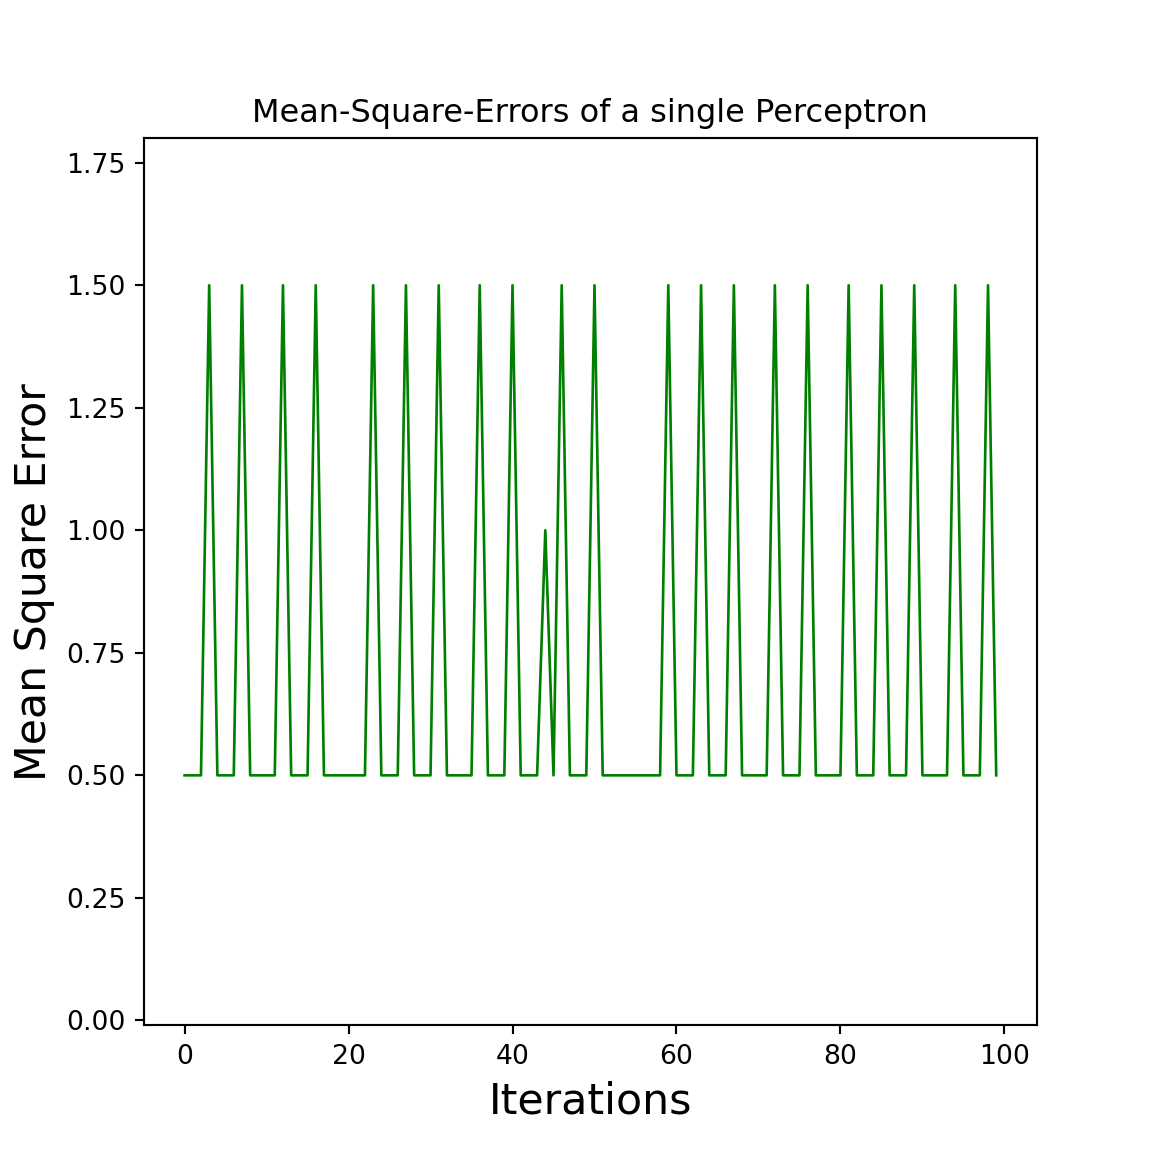
\includegraphics{gitbook-demo_files/figure-latex/unnamed-chunk-14-3.pdf}

\hypertarget{multi-layer-perceptrons}{%
\chapter{Multi Layer Perceptrons}\label{multi-layer-perceptrons}}

In a multi layer Perceptron you have multiple layers of neurons. Thats why you need to calculate the forward pass multiple times and the same for the backward pass. First of all, do we need to generalise some definitions, to support this behavior. You can interprete each layer as a single Perceptron.

  \bibliography{book.bib,packages.bib}

\end{document}
